\documentclass[11pt]{article}
\usepackage[textwidth=18.0cm, textheight=23.0cm, top=2.0cm]{geometry}
\usepackage{pst-all}
\usepackage{amssymb}
\usepackage{tikz}
\usepackage{underscore}\begin{document}
\pagestyle{empty}


ClassName: \underline{\textbf{Class_05.2bp-26}}
\par
BinSize: \underline{\textbf{100 × 100}}
\par
ReduceSize: \underline{\textbf{100 × 100}}
\par
TypeNum: \underline{\textbf{60}}
\par
Num: \underline{\textbf{60}}
\par
OutS: \underline{\textbf{140000}}
\par
InS: \underline{\textbf{124587}}
\par
Rate: \underline{\textbf{0.890}}
\par
UB: \underline{\textbf{14}}
\par
LB0: \underline{\textbf{14}}
\par
LB: \underline{\textbf{14}}
\par
LBWithCut: \underline{\textbf{14}}
\par
NodeCut: \underline{\textbf{0}}
\par
ExtendedNodeCnt: \underline{\textbf{1}}
\par
GenNodeCnt: \underline{\textbf{1}}
\par
PrimalNode: \underline{\textbf{0}}
\par
ColumnCount: \underline{\textbf{14}}
\par
TotalCutCount: \underline{\textbf{0}}
\par
RootCutCount: \underline{\textbf{0}}
\par
LPSolverCnt: \underline{\textbf{1}}
\par
PricingSolverCnt: \underline{\textbf{0}}
\par
BranchAndBoundNum: \underline{\textbf{1}}
\par
isOpt: \underline{\textbf{true}}
\par
TimeOnPrimal: \underline{\textbf{0.000 s}}
\par
TimeOnPricing: \underline{\textbf{0.000 s}}
\par
TimeOnRmp: \underline{\textbf{0.078 s}}
\par
TotalTime: \underline{\textbf{0.141 s}}
\par
\newpage


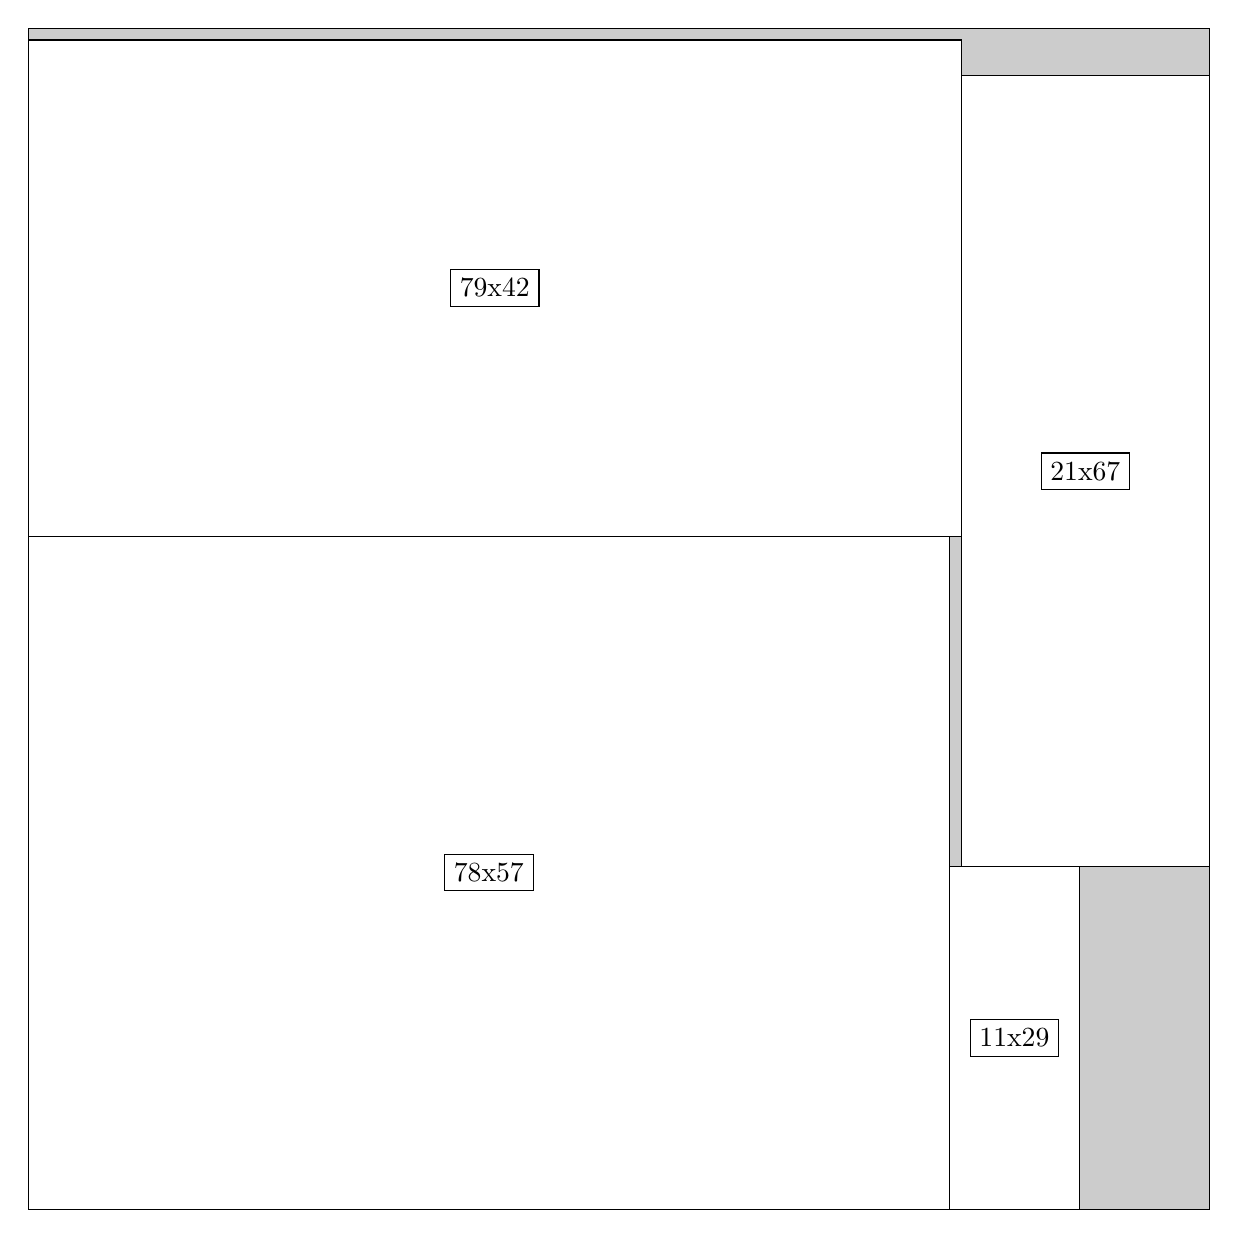
\begin{tikzpicture}[shorten >=1pt,scale=1.0,every node/.style={scale=1.0},->]
\tikzstyle{vertex}=[circle,fill=black!25,minimum size=14pt,inner sep=0pt]
\filldraw[fill=gray!40!white, draw=black] (0,0) rectangle (15.0,15.0);
\foreach \name/\x/\y/\w/\h in {11x29/11.7/0.0/1.65/4.35,78x57/0.0/0.0/11.7/8.549999999999999,79x42/0.0/8.549999999999999/11.85/6.3,21x67/11.85/4.35/3.15/10.049999999999999}
\filldraw[fill=white!40!white, draw=black] (\x,\y) rectangle node[draw] (\name) {\name} ++(\w,\h);
\end{tikzpicture}


w =11 , h =29 , x =78 , y =0 , v =319
\par
w =78 , h =57 , x =0 , y =0 , v =4446
\par
w =79 , h =42 , x =0 , y =57 , v =3318
\par
w =21 , h =67 , x =79 , y =29 , v =1407
\par
\newpage


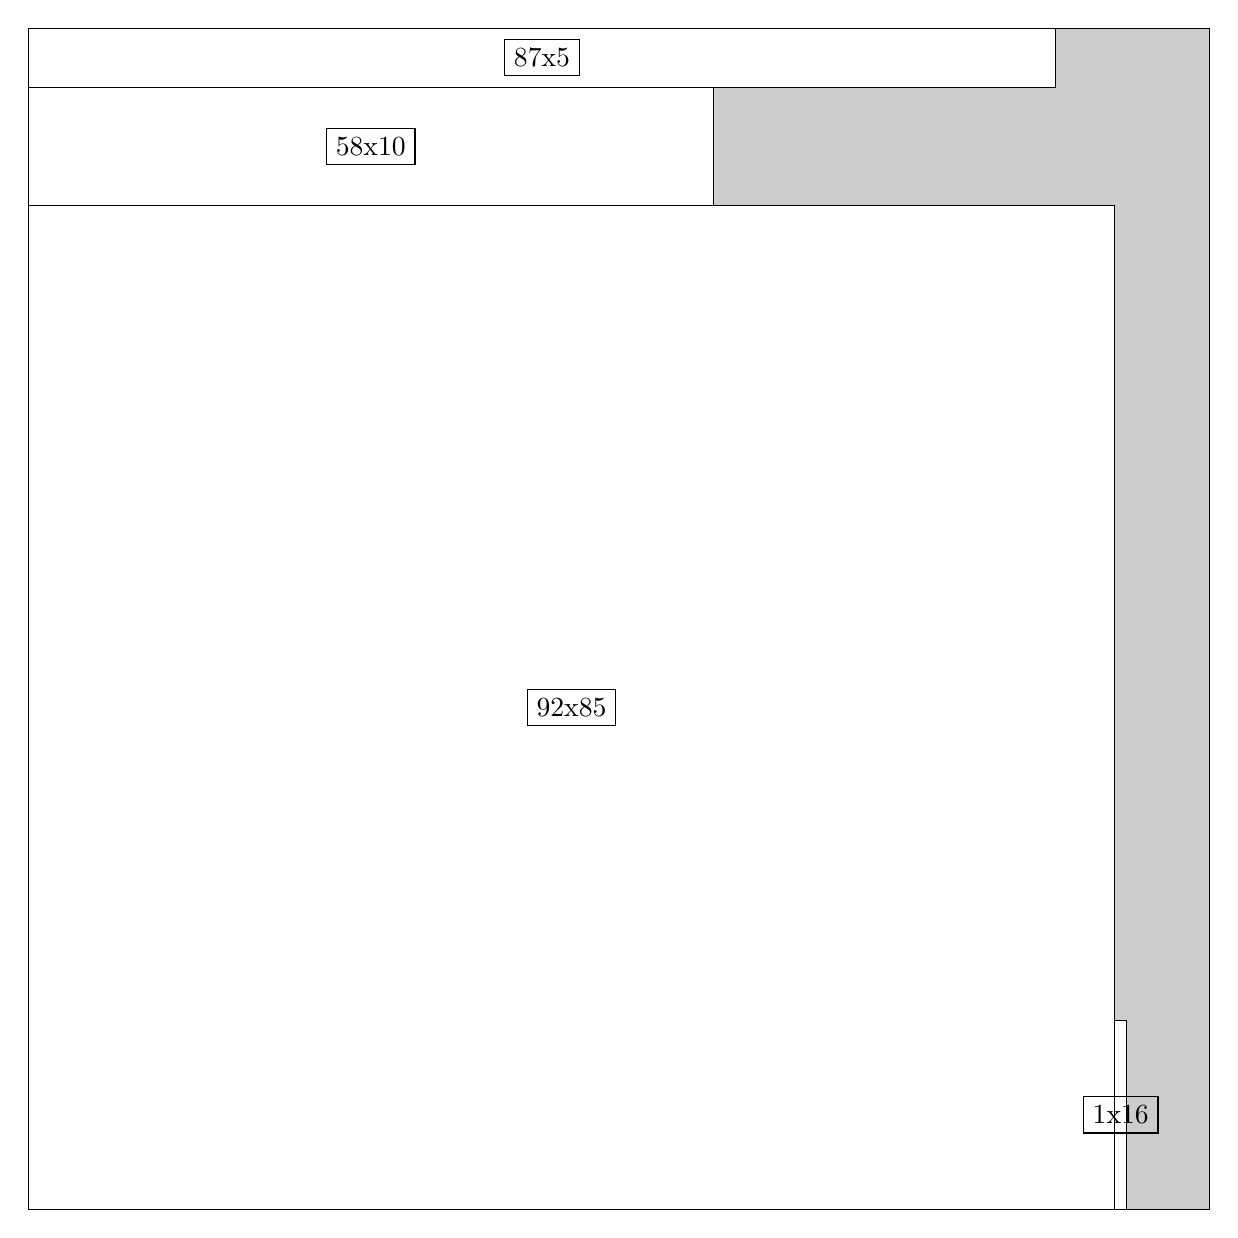
\begin{tikzpicture}[shorten >=1pt,scale=1.0,every node/.style={scale=1.0},->]
\tikzstyle{vertex}=[circle,fill=black!25,minimum size=14pt,inner sep=0pt]
\filldraw[fill=gray!40!white, draw=black] (0,0) rectangle (15.0,15.0);
\foreach \name/\x/\y/\w/\h in {92x85/0.0/0.0/13.799999999999999/12.75,58x10/0.0/12.75/8.7/1.5,87x5/0.0/14.25/13.049999999999999/0.75,1x16/13.799999999999999/0.0/0.15/2.4}
\filldraw[fill=white!40!white, draw=black] (\x,\y) rectangle node[draw] (\name) {\name} ++(\w,\h);
\end{tikzpicture}


w =92 , h =85 , x =0 , y =0 , v =7820
\par
w =58 , h =10 , x =0 , y =85 , v =580
\par
w =87 , h =5 , x =0 , y =95 , v =435
\par
w =1 , h =16 , x =92 , y =0 , v =16
\par
\newpage


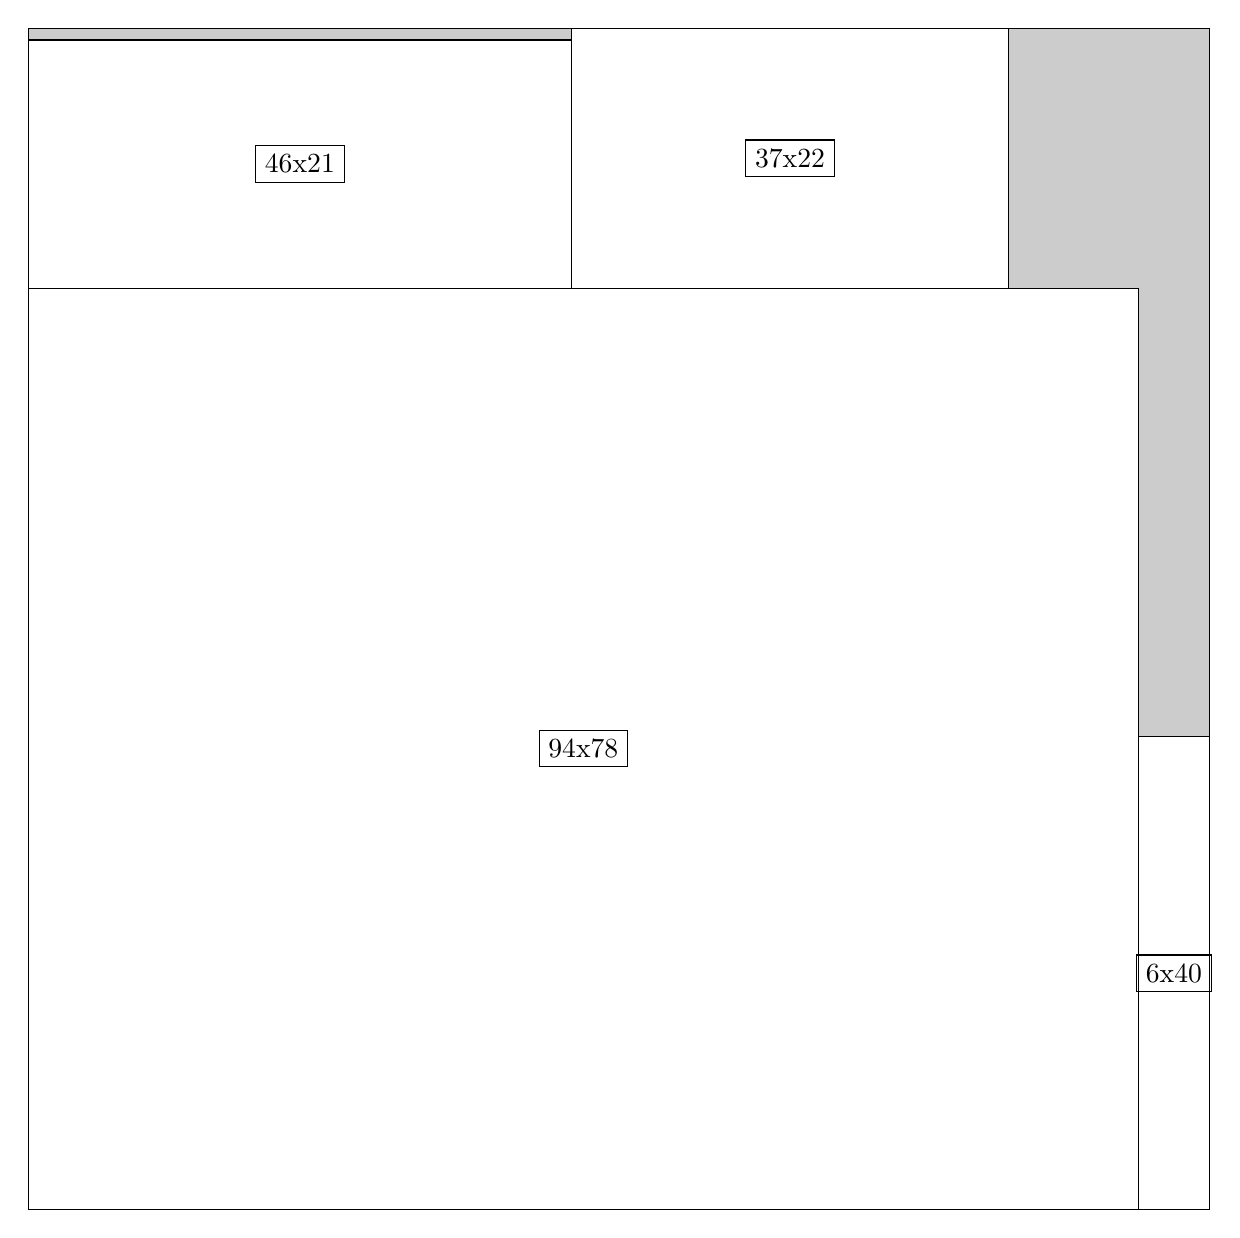
\begin{tikzpicture}[shorten >=1pt,scale=1.0,every node/.style={scale=1.0},->]
\tikzstyle{vertex}=[circle,fill=black!25,minimum size=14pt,inner sep=0pt]
\filldraw[fill=gray!40!white, draw=black] (0,0) rectangle (15.0,15.0);
\foreach \name/\x/\y/\w/\h in {94x78/0.0/0.0/14.1/11.7,46x21/0.0/11.7/6.8999999999999995/3.15,37x22/6.8999999999999995/11.7/5.55/3.3,6x40/14.1/0.0/0.8999999999999999/6.0}
\filldraw[fill=white!40!white, draw=black] (\x,\y) rectangle node[draw] (\name) {\name} ++(\w,\h);
\end{tikzpicture}


w =94 , h =78 , x =0 , y =0 , v =7332
\par
w =46 , h =21 , x =0 , y =78 , v =966
\par
w =37 , h =22 , x =46 , y =78 , v =814
\par
w =6 , h =40 , x =94 , y =0 , v =240
\par
\newpage


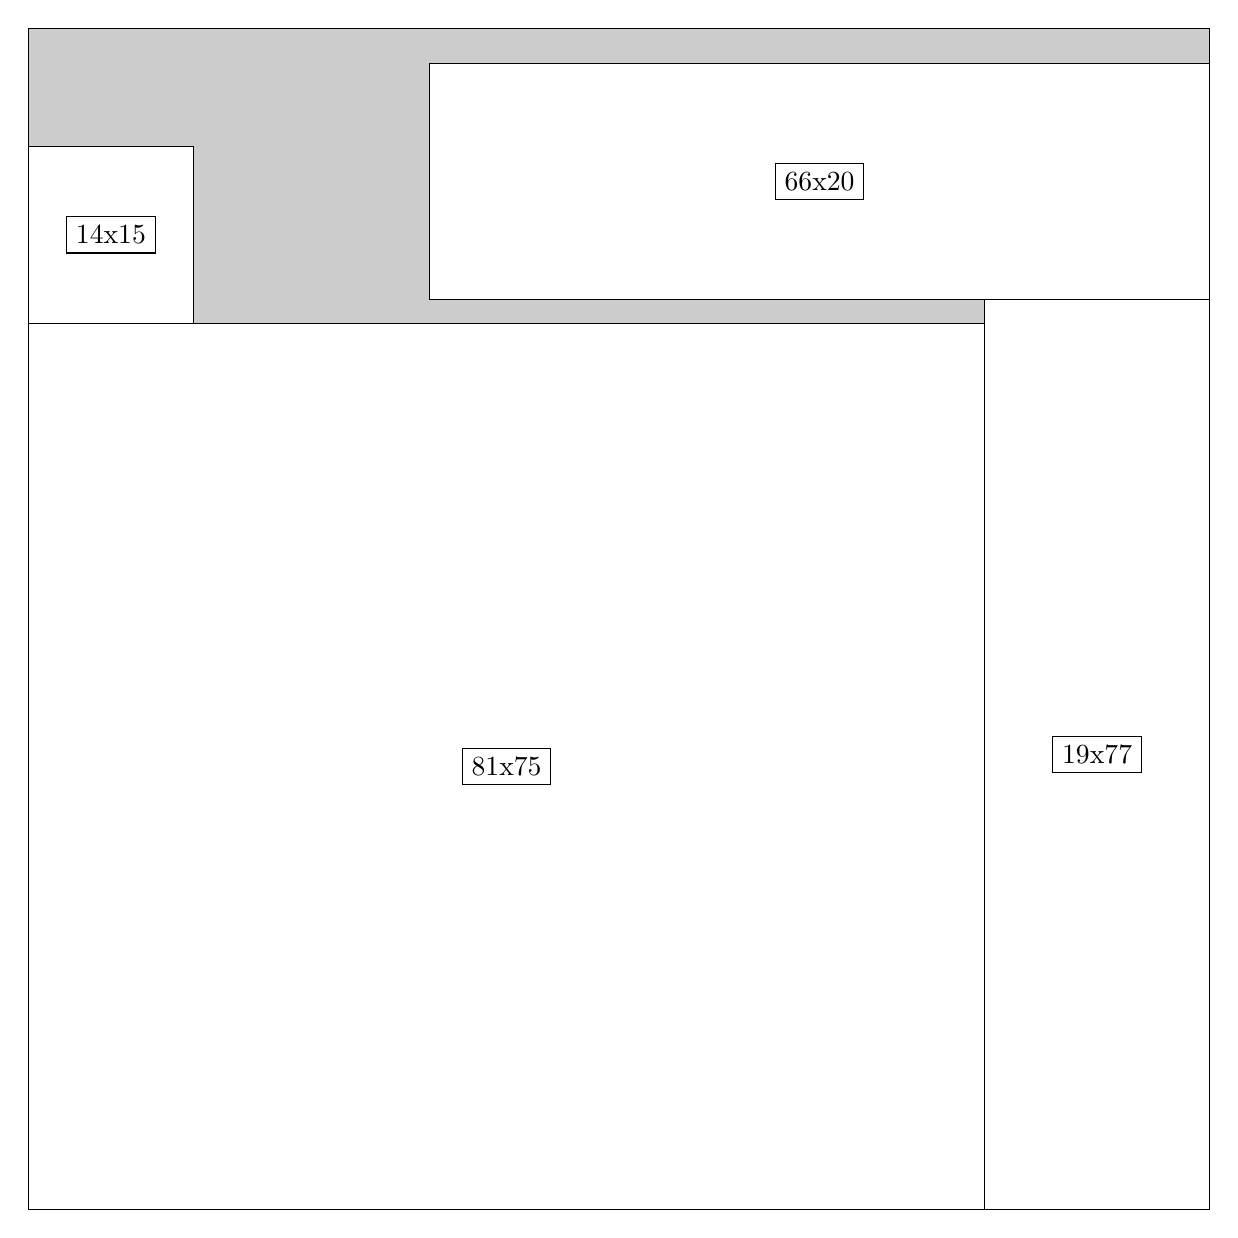
\begin{tikzpicture}[shorten >=1pt,scale=1.0,every node/.style={scale=1.0},->]
\tikzstyle{vertex}=[circle,fill=black!25,minimum size=14pt,inner sep=0pt]
\filldraw[fill=gray!40!white, draw=black] (0,0) rectangle (15.0,15.0);
\foreach \name/\x/\y/\w/\h in {81x75/0.0/0.0/12.15/11.25,19x77/12.15/0.0/2.85/11.549999999999999,66x20/5.1/11.549999999999999/9.9/3.0,14x15/0.0/11.25/2.1/2.25}
\filldraw[fill=white!40!white, draw=black] (\x,\y) rectangle node[draw] (\name) {\name} ++(\w,\h);
\end{tikzpicture}


w =81 , h =75 , x =0 , y =0 , v =6075
\par
w =19 , h =77 , x =81 , y =0 , v =1463
\par
w =66 , h =20 , x =34 , y =77 , v =1320
\par
w =14 , h =15 , x =0 , y =75 , v =210
\par
\newpage


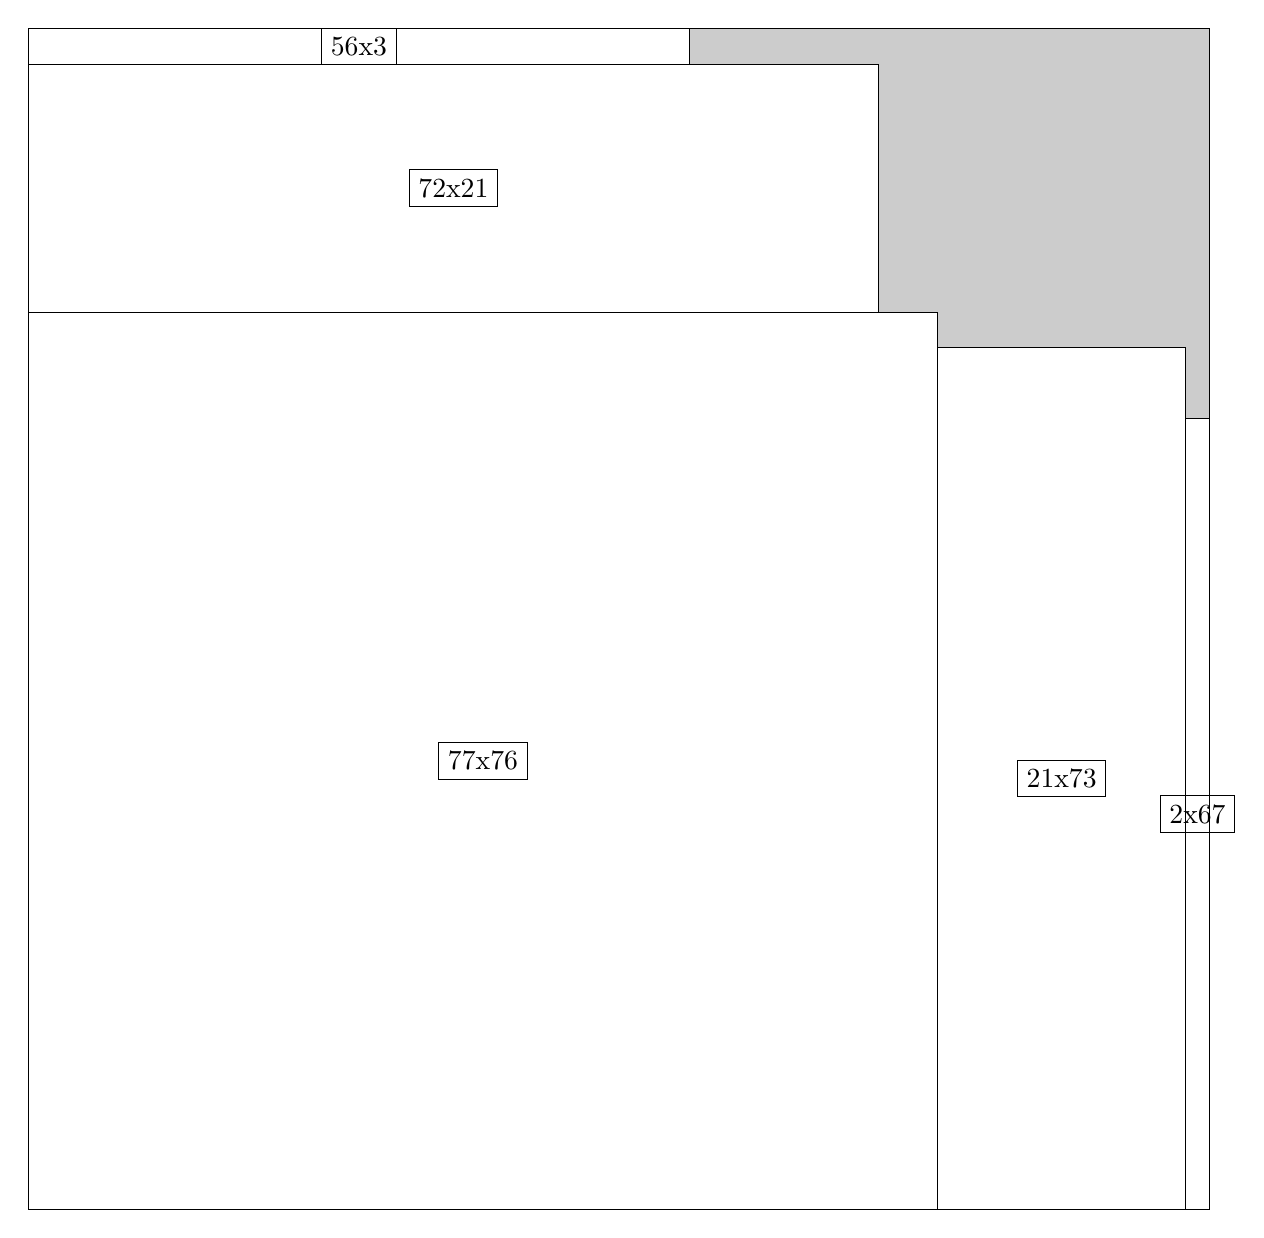
\begin{tikzpicture}[shorten >=1pt,scale=1.0,every node/.style={scale=1.0},->]
\tikzstyle{vertex}=[circle,fill=black!25,minimum size=14pt,inner sep=0pt]
\filldraw[fill=gray!40!white, draw=black] (0,0) rectangle (15.0,15.0);
\foreach \name/\x/\y/\w/\h in {77x76/0.0/0.0/11.549999999999999/11.4,21x73/11.549999999999999/0.0/3.15/10.95,72x21/0.0/11.4/10.799999999999999/3.15,56x3/0.0/14.549999999999999/8.4/0.44999999999999996,2x67/14.7/0.0/0.3/10.049999999999999}
\filldraw[fill=white!40!white, draw=black] (\x,\y) rectangle node[draw] (\name) {\name} ++(\w,\h);
\end{tikzpicture}


w =77 , h =76 , x =0 , y =0 , v =5852
\par
w =21 , h =73 , x =77 , y =0 , v =1533
\par
w =72 , h =21 , x =0 , y =76 , v =1512
\par
w =56 , h =3 , x =0 , y =97 , v =168
\par
w =2 , h =67 , x =98 , y =0 , v =134
\par
\newpage


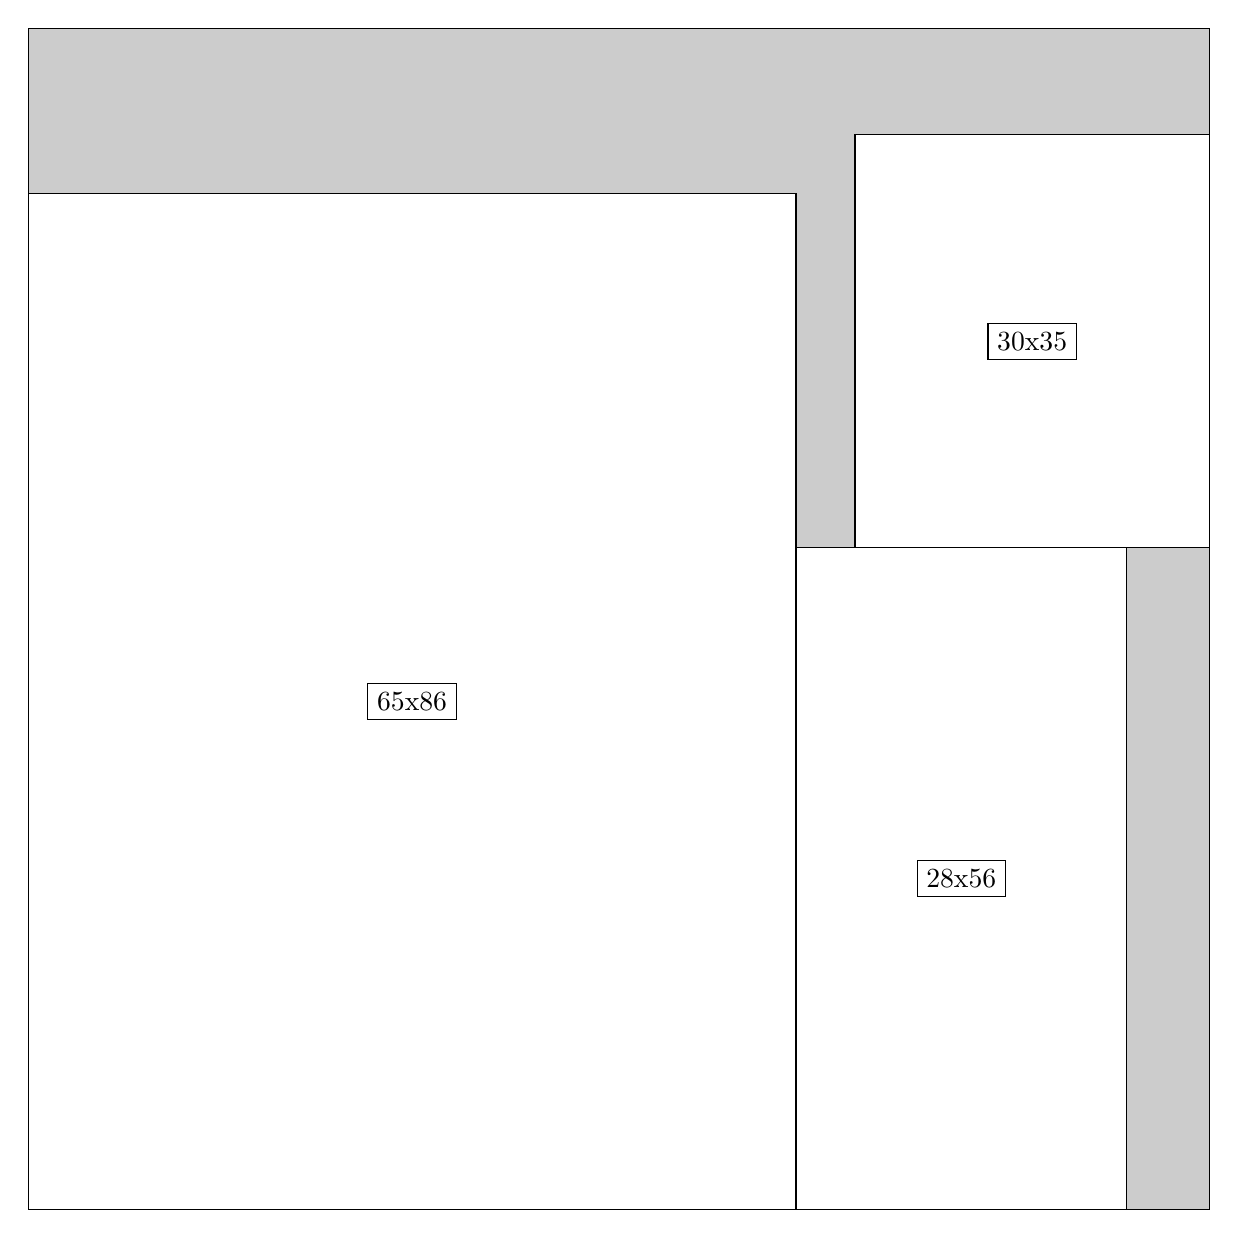
\begin{tikzpicture}[shorten >=1pt,scale=1.0,every node/.style={scale=1.0},->]
\tikzstyle{vertex}=[circle,fill=black!25,minimum size=14pt,inner sep=0pt]
\filldraw[fill=gray!40!white, draw=black] (0,0) rectangle (15.0,15.0);
\foreach \name/\x/\y/\w/\h in {65x86/0.0/0.0/9.75/12.9,28x56/9.75/0.0/4.2/8.4,30x35/10.5/8.4/4.5/5.25}
\filldraw[fill=white!40!white, draw=black] (\x,\y) rectangle node[draw] (\name) {\name} ++(\w,\h);
\end{tikzpicture}


w =65 , h =86 , x =0 , y =0 , v =5590
\par
w =28 , h =56 , x =65 , y =0 , v =1568
\par
w =30 , h =35 , x =70 , y =56 , v =1050
\par
\newpage


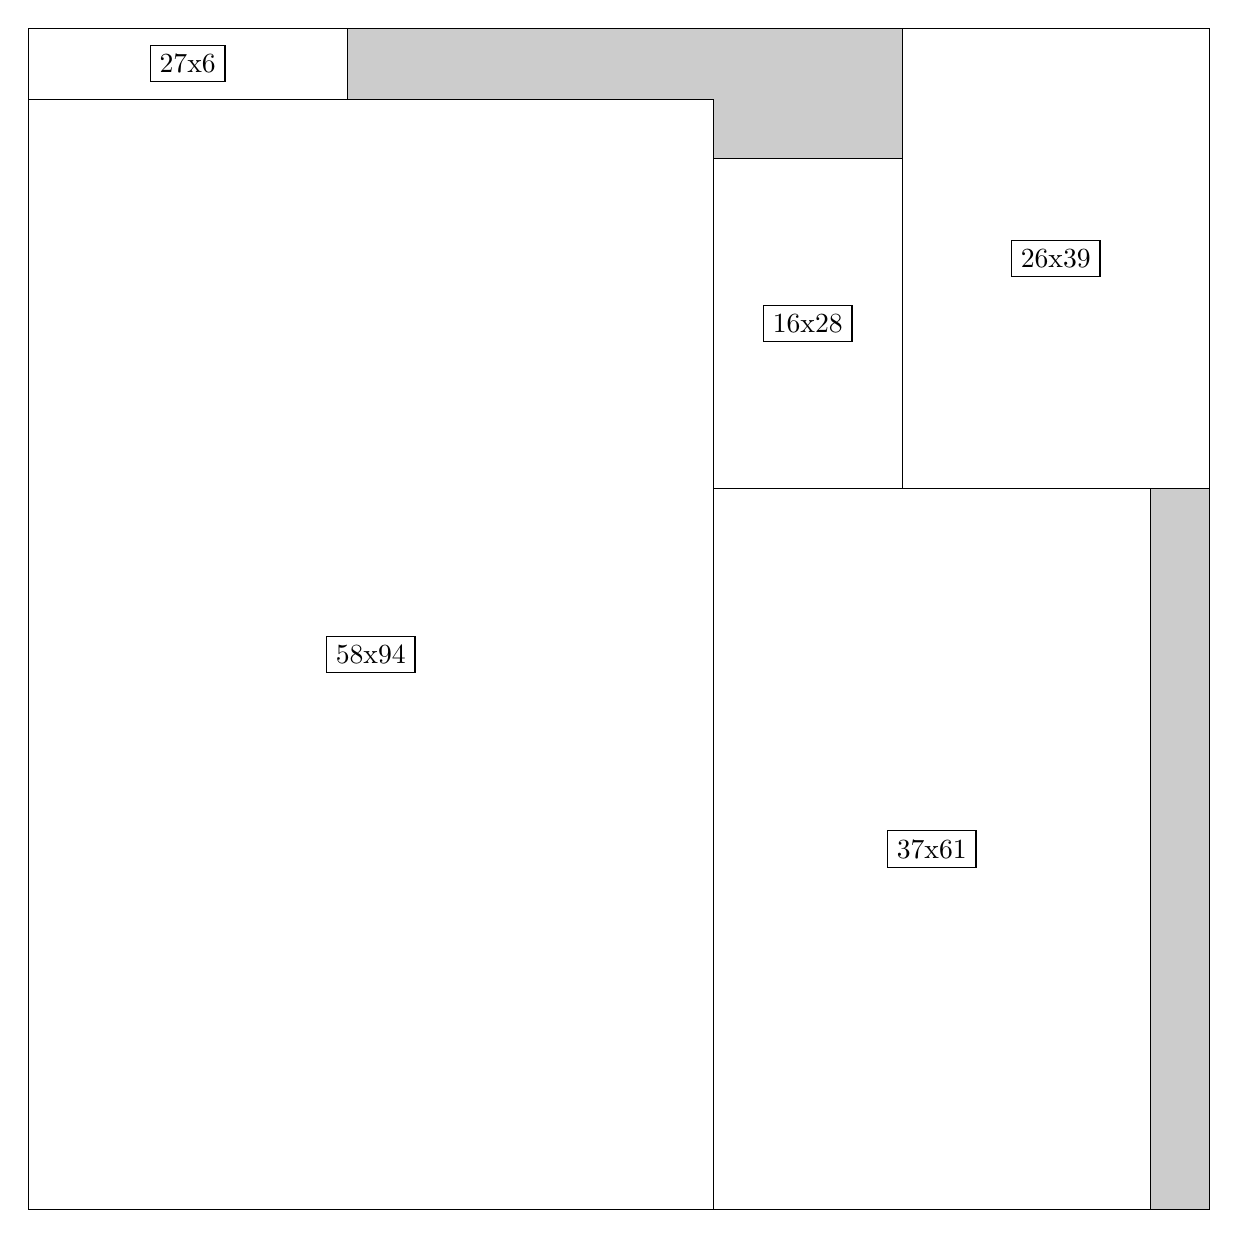
\begin{tikzpicture}[shorten >=1pt,scale=1.0,every node/.style={scale=1.0},->]
\tikzstyle{vertex}=[circle,fill=black!25,minimum size=14pt,inner sep=0pt]
\filldraw[fill=gray!40!white, draw=black] (0,0) rectangle (15.0,15.0);
\foreach \name/\x/\y/\w/\h in {58x94/0.0/0.0/8.7/14.1,37x61/8.7/0.0/5.55/9.15,26x39/11.1/9.15/3.9/5.85,16x28/8.7/9.15/2.4/4.2,27x6/0.0/14.1/4.05/0.8999999999999999}
\filldraw[fill=white!40!white, draw=black] (\x,\y) rectangle node[draw] (\name) {\name} ++(\w,\h);
\end{tikzpicture}


w =58 , h =94 , x =0 , y =0 , v =5452
\par
w =37 , h =61 , x =58 , y =0 , v =2257
\par
w =26 , h =39 , x =74 , y =61 , v =1014
\par
w =16 , h =28 , x =58 , y =61 , v =448
\par
w =27 , h =6 , x =0 , y =94 , v =162
\par
\newpage


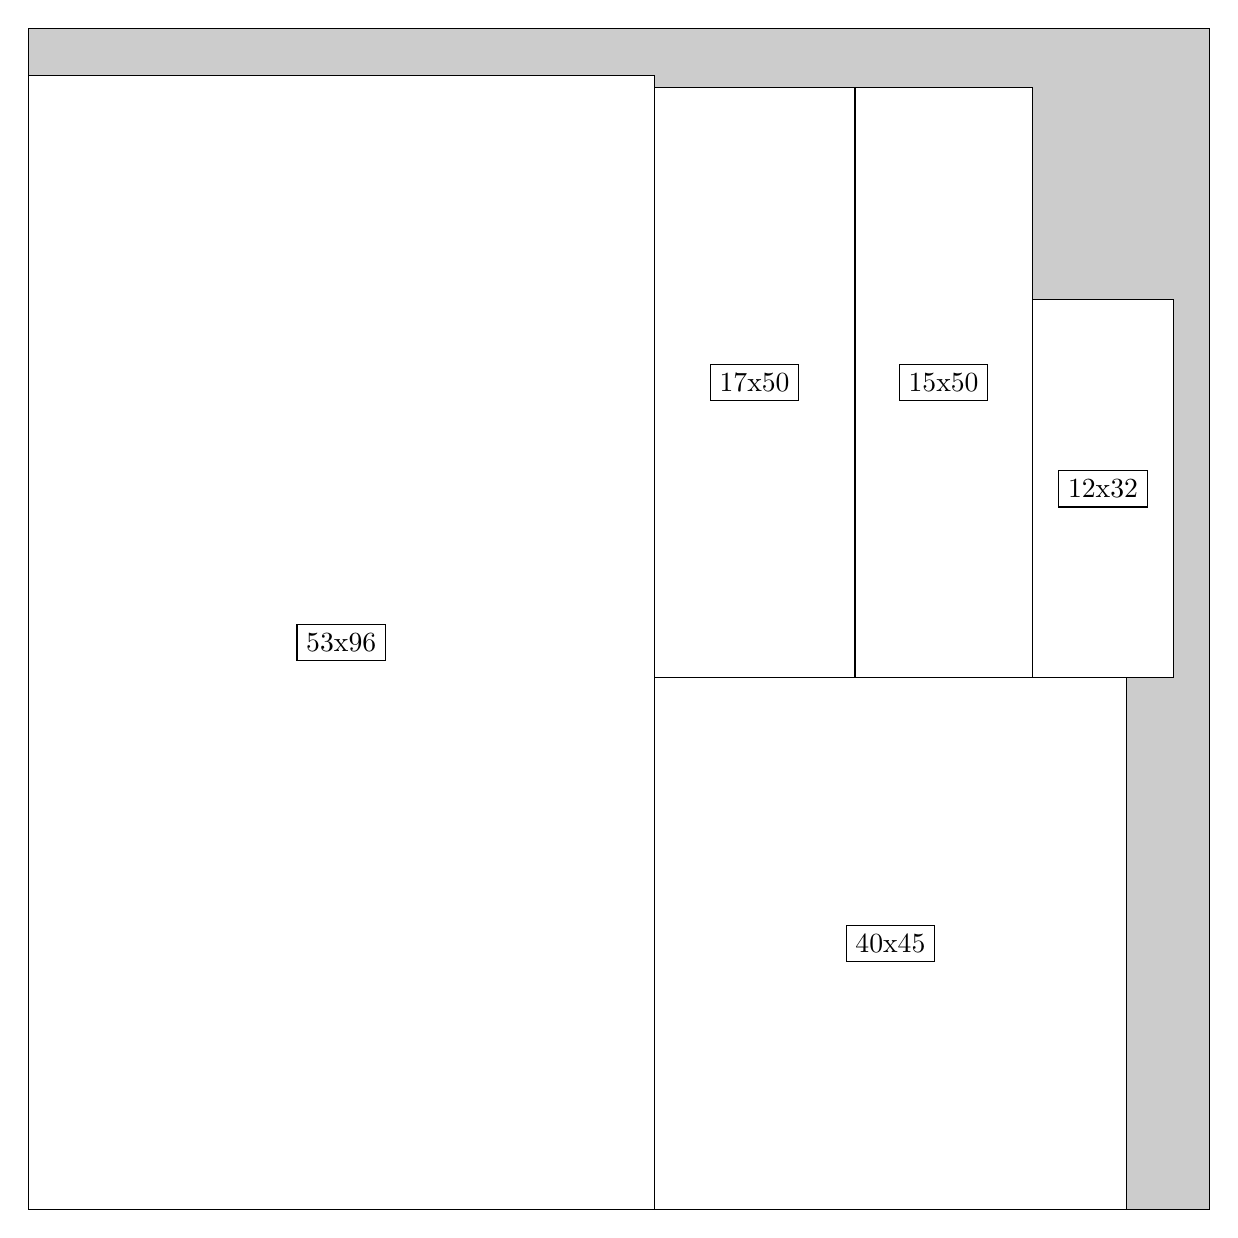
\begin{tikzpicture}[shorten >=1pt,scale=1.0,every node/.style={scale=1.0},->]
\tikzstyle{vertex}=[circle,fill=black!25,minimum size=14pt,inner sep=0pt]
\filldraw[fill=gray!40!white, draw=black] (0,0) rectangle (15.0,15.0);
\foreach \name/\x/\y/\w/\h in {53x96/0.0/0.0/7.949999999999999/14.399999999999999,40x45/7.949999999999999/0.0/6.0/6.75,17x50/7.949999999999999/6.75/2.55/7.5,15x50/10.5/6.75/2.25/7.5,12x32/12.75/6.75/1.7999999999999998/4.8}
\filldraw[fill=white!40!white, draw=black] (\x,\y) rectangle node[draw] (\name) {\name} ++(\w,\h);
\end{tikzpicture}


w =53 , h =96 , x =0 , y =0 , v =5088
\par
w =40 , h =45 , x =53 , y =0 , v =1800
\par
w =17 , h =50 , x =53 , y =45 , v =850
\par
w =15 , h =50 , x =70 , y =45 , v =750
\par
w =12 , h =32 , x =85 , y =45 , v =384
\par
\newpage


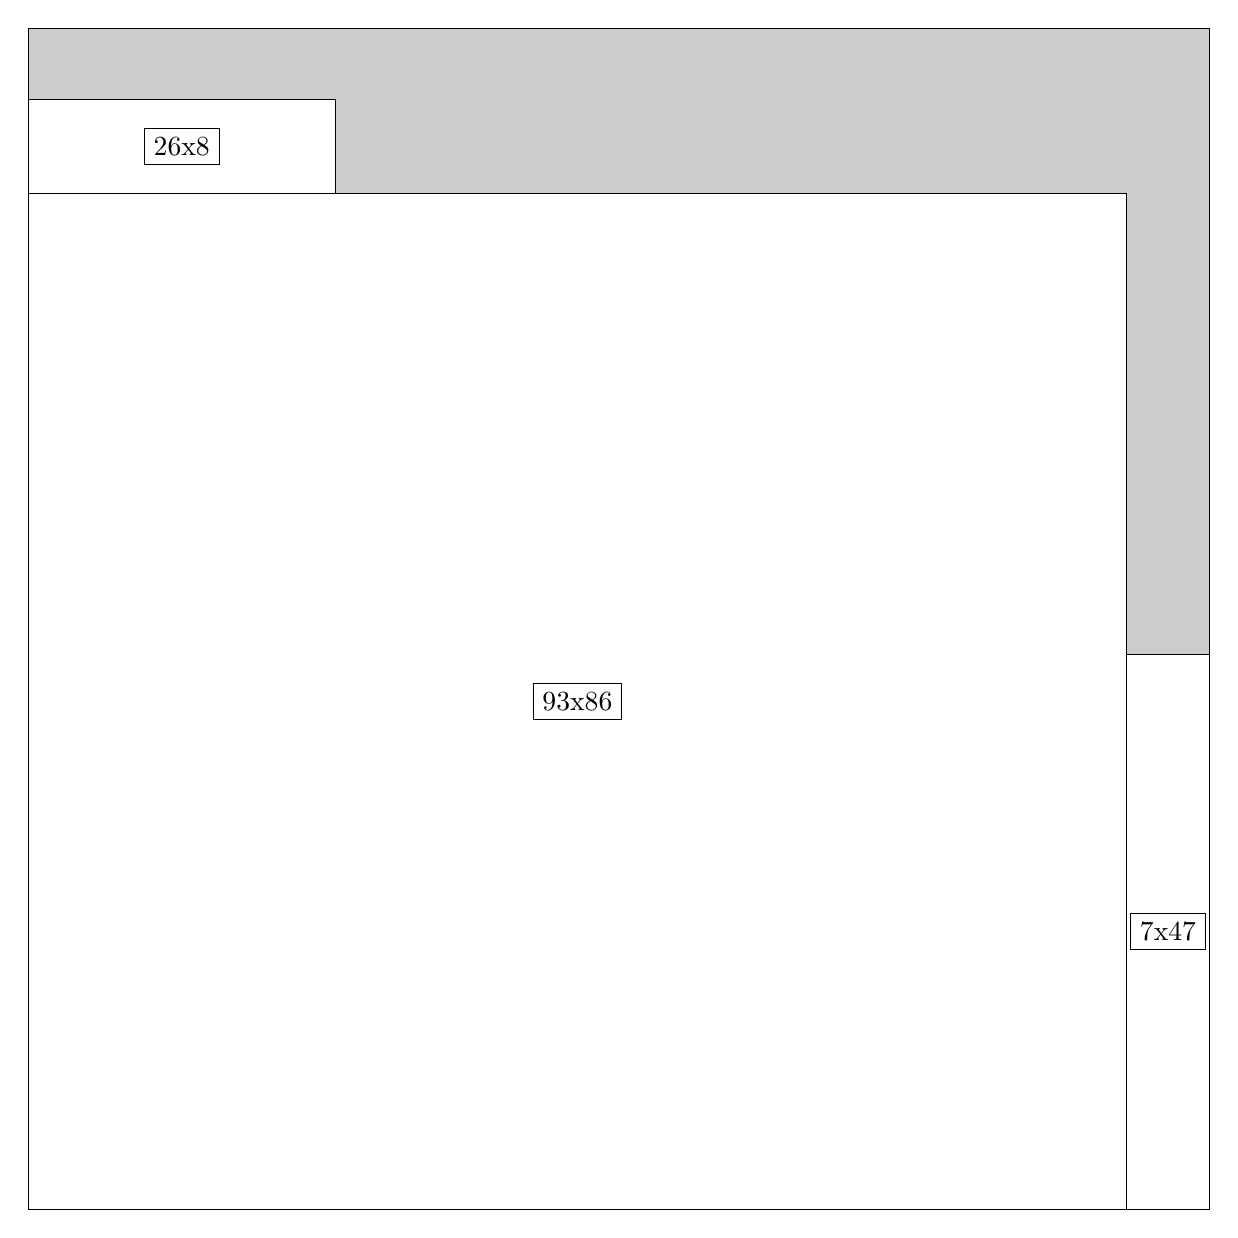
\begin{tikzpicture}[shorten >=1pt,scale=1.0,every node/.style={scale=1.0},->]
\tikzstyle{vertex}=[circle,fill=black!25,minimum size=14pt,inner sep=0pt]
\filldraw[fill=gray!40!white, draw=black] (0,0) rectangle (15.0,15.0);
\foreach \name/\x/\y/\w/\h in {7x47/13.95/0.0/1.05/7.05,93x86/0.0/0.0/13.95/12.9,26x8/0.0/12.9/3.9/1.2}
\filldraw[fill=white!40!white, draw=black] (\x,\y) rectangle node[draw] (\name) {\name} ++(\w,\h);
\end{tikzpicture}


w =7 , h =47 , x =93 , y =0 , v =329
\par
w =93 , h =86 , x =0 , y =0 , v =7998
\par
w =26 , h =8 , x =0 , y =86 , v =208
\par
\newpage


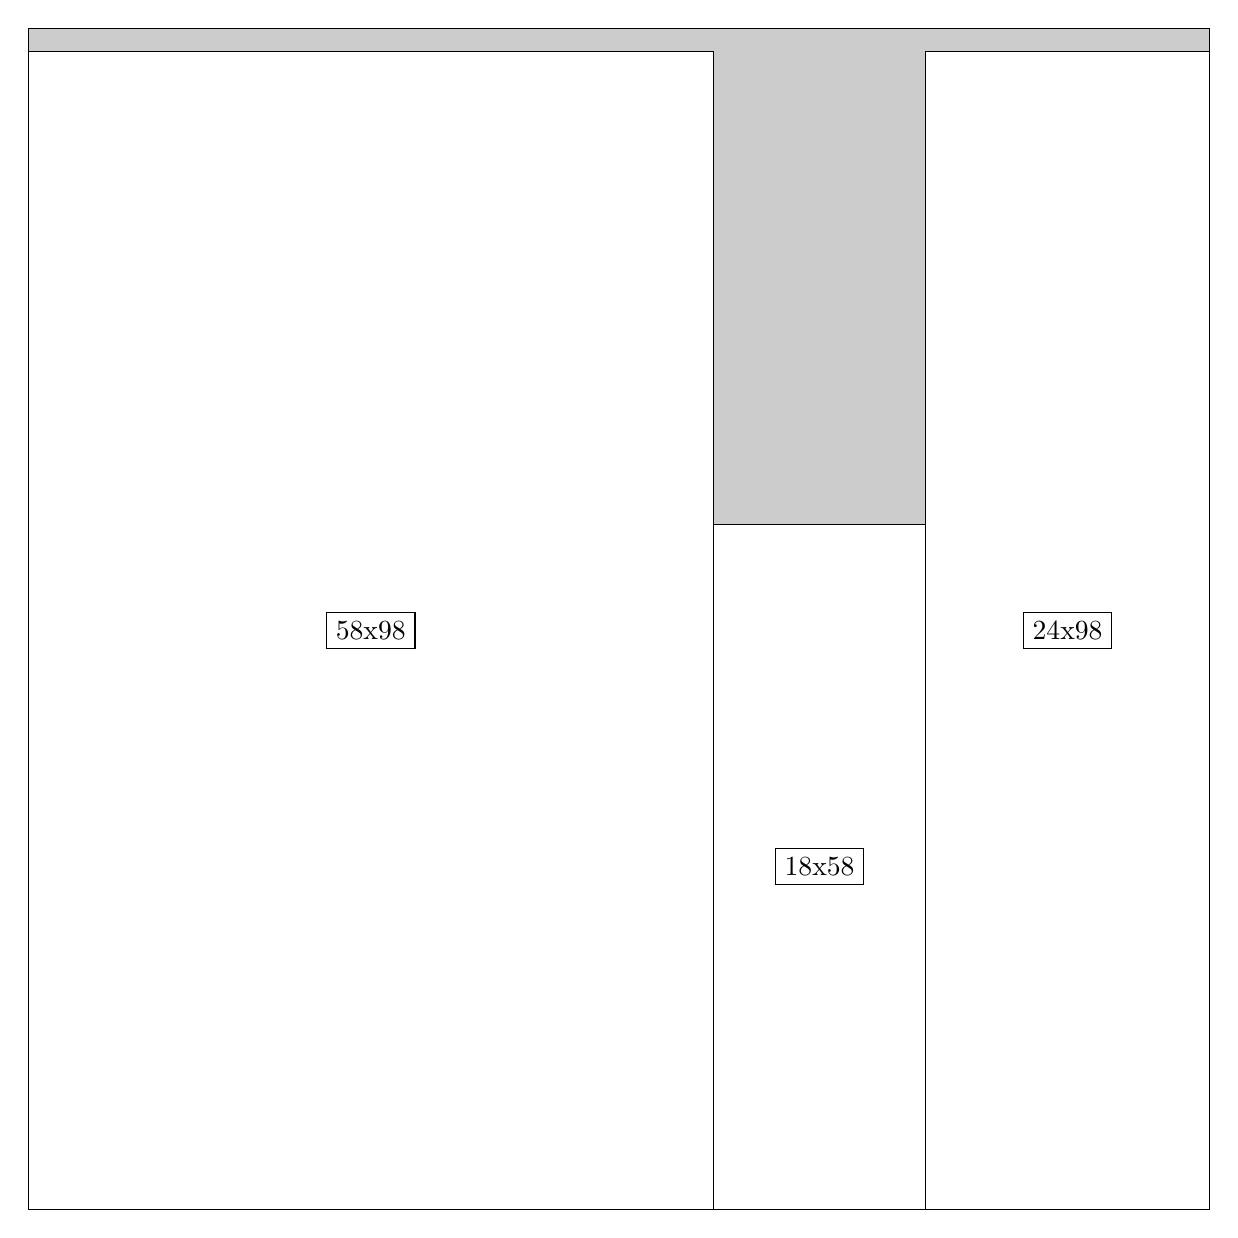
\begin{tikzpicture}[shorten >=1pt,scale=1.0,every node/.style={scale=1.0},->]
\tikzstyle{vertex}=[circle,fill=black!25,minimum size=14pt,inner sep=0pt]
\filldraw[fill=gray!40!white, draw=black] (0,0) rectangle (15.0,15.0);
\foreach \name/\x/\y/\w/\h in {58x98/0.0/0.0/8.7/14.7,24x98/11.4/0.0/3.5999999999999996/14.7,18x58/8.7/0.0/2.6999999999999997/8.7}
\filldraw[fill=white!40!white, draw=black] (\x,\y) rectangle node[draw] (\name) {\name} ++(\w,\h);
\end{tikzpicture}


w =58 , h =98 , x =0 , y =0 , v =5684
\par
w =24 , h =98 , x =76 , y =0 , v =2352
\par
w =18 , h =58 , x =58 , y =0 , v =1044
\par
\newpage


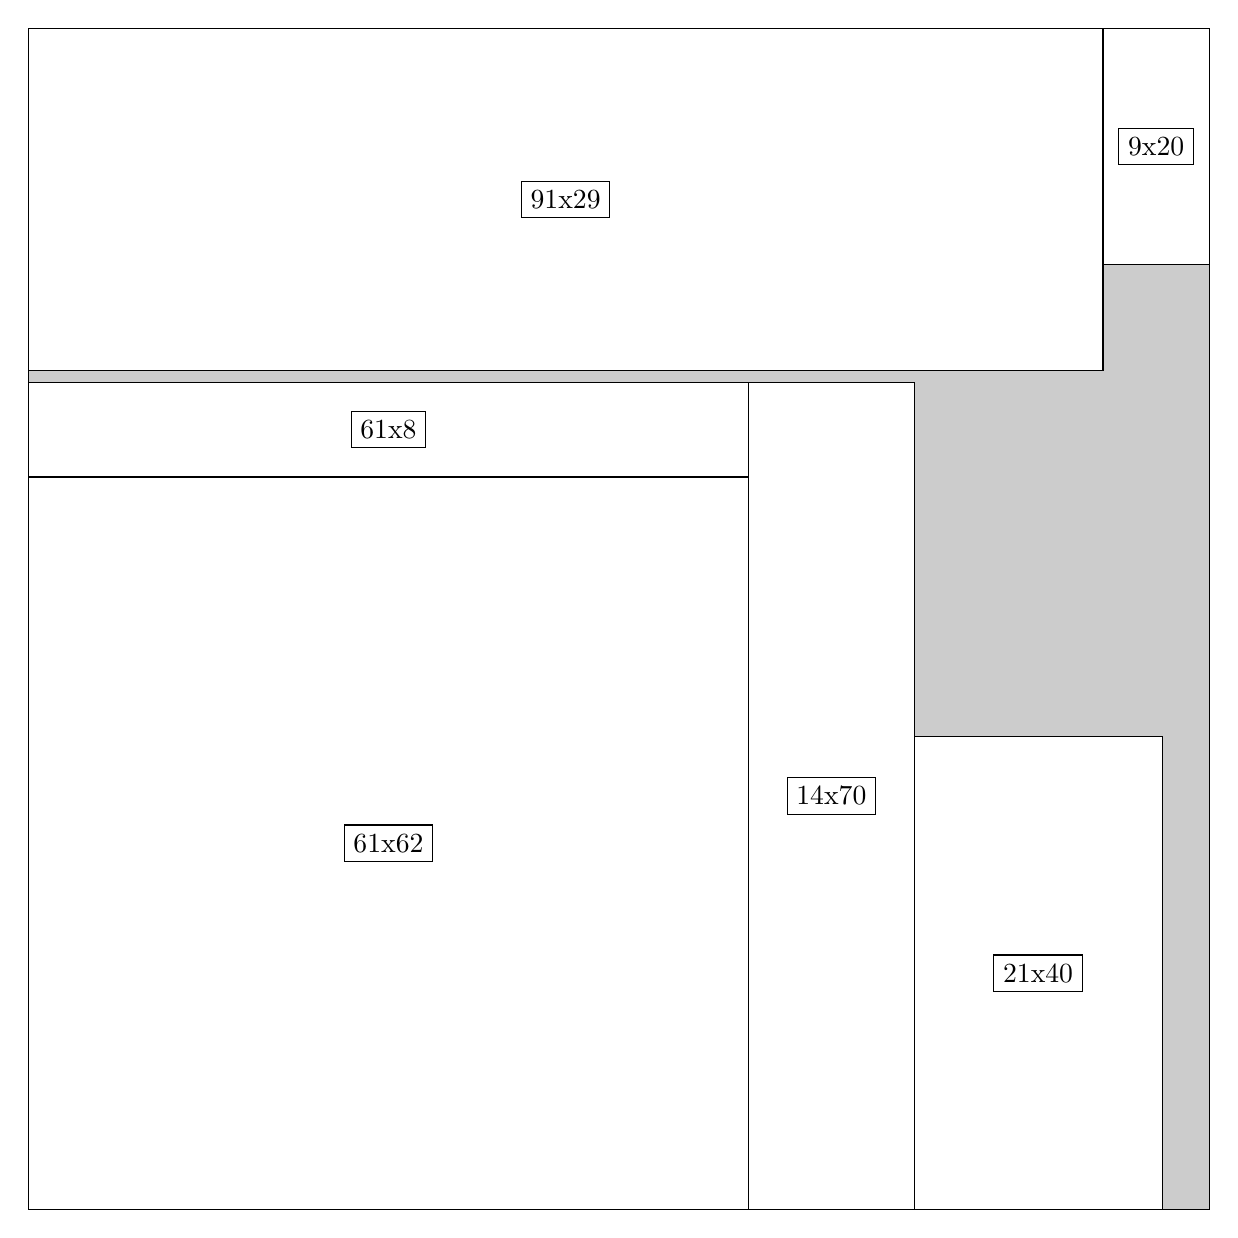
\begin{tikzpicture}[shorten >=1pt,scale=1.0,every node/.style={scale=1.0},->]
\tikzstyle{vertex}=[circle,fill=black!25,minimum size=14pt,inner sep=0pt]
\filldraw[fill=gray!40!white, draw=black] (0,0) rectangle (15.0,15.0);
\foreach \name/\x/\y/\w/\h in {61x62/0.0/0.0/9.15/9.299999999999999,91x29/0.0/10.65/13.65/4.35,14x70/9.15/0.0/2.1/10.5,21x40/11.25/0.0/3.15/6.0,61x8/0.0/9.299999999999999/9.15/1.2,9x20/13.65/12.0/1.3499999999999999/3.0}
\filldraw[fill=white!40!white, draw=black] (\x,\y) rectangle node[draw] (\name) {\name} ++(\w,\h);
\end{tikzpicture}


w =61 , h =62 , x =0 , y =0 , v =3782
\par
w =91 , h =29 , x =0 , y =71 , v =2639
\par
w =14 , h =70 , x =61 , y =0 , v =980
\par
w =21 , h =40 , x =75 , y =0 , v =840
\par
w =61 , h =8 , x =0 , y =62 , v =488
\par
w =9 , h =20 , x =91 , y =80 , v =180
\par
\newpage


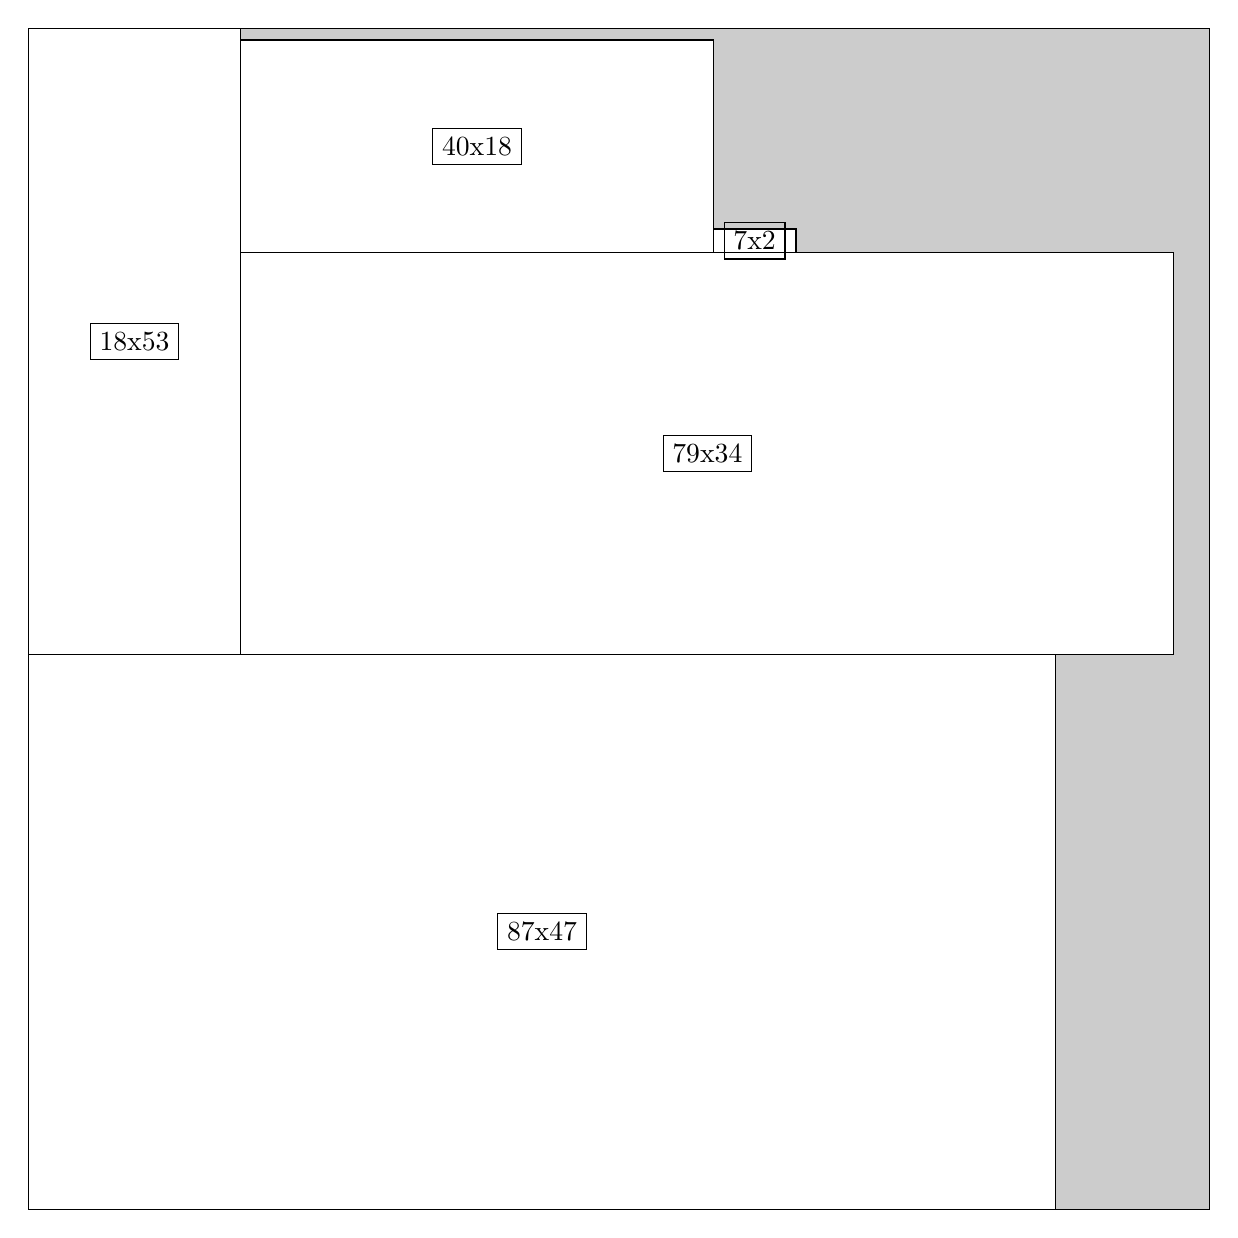
\begin{tikzpicture}[shorten >=1pt,scale=1.0,every node/.style={scale=1.0},->]
\tikzstyle{vertex}=[circle,fill=black!25,minimum size=14pt,inner sep=0pt]
\filldraw[fill=gray!40!white, draw=black] (0,0) rectangle (15.0,15.0);
\foreach \name/\x/\y/\w/\h in {87x47/0.0/0.0/13.049999999999999/7.05,79x34/2.6999999999999997/7.05/11.85/5.1,18x53/0.0/7.05/2.6999999999999997/7.949999999999999,40x18/2.6999999999999997/12.15/6.0/2.6999999999999997,7x2/8.7/12.15/1.05/0.3}
\filldraw[fill=white!40!white, draw=black] (\x,\y) rectangle node[draw] (\name) {\name} ++(\w,\h);
\end{tikzpicture}


w =87 , h =47 , x =0 , y =0 , v =4089
\par
w =79 , h =34 , x =18 , y =47 , v =2686
\par
w =18 , h =53 , x =0 , y =47 , v =954
\par
w =40 , h =18 , x =18 , y =81 , v =720
\par
w =7 , h =2 , x =58 , y =81 , v =14
\par
\newpage


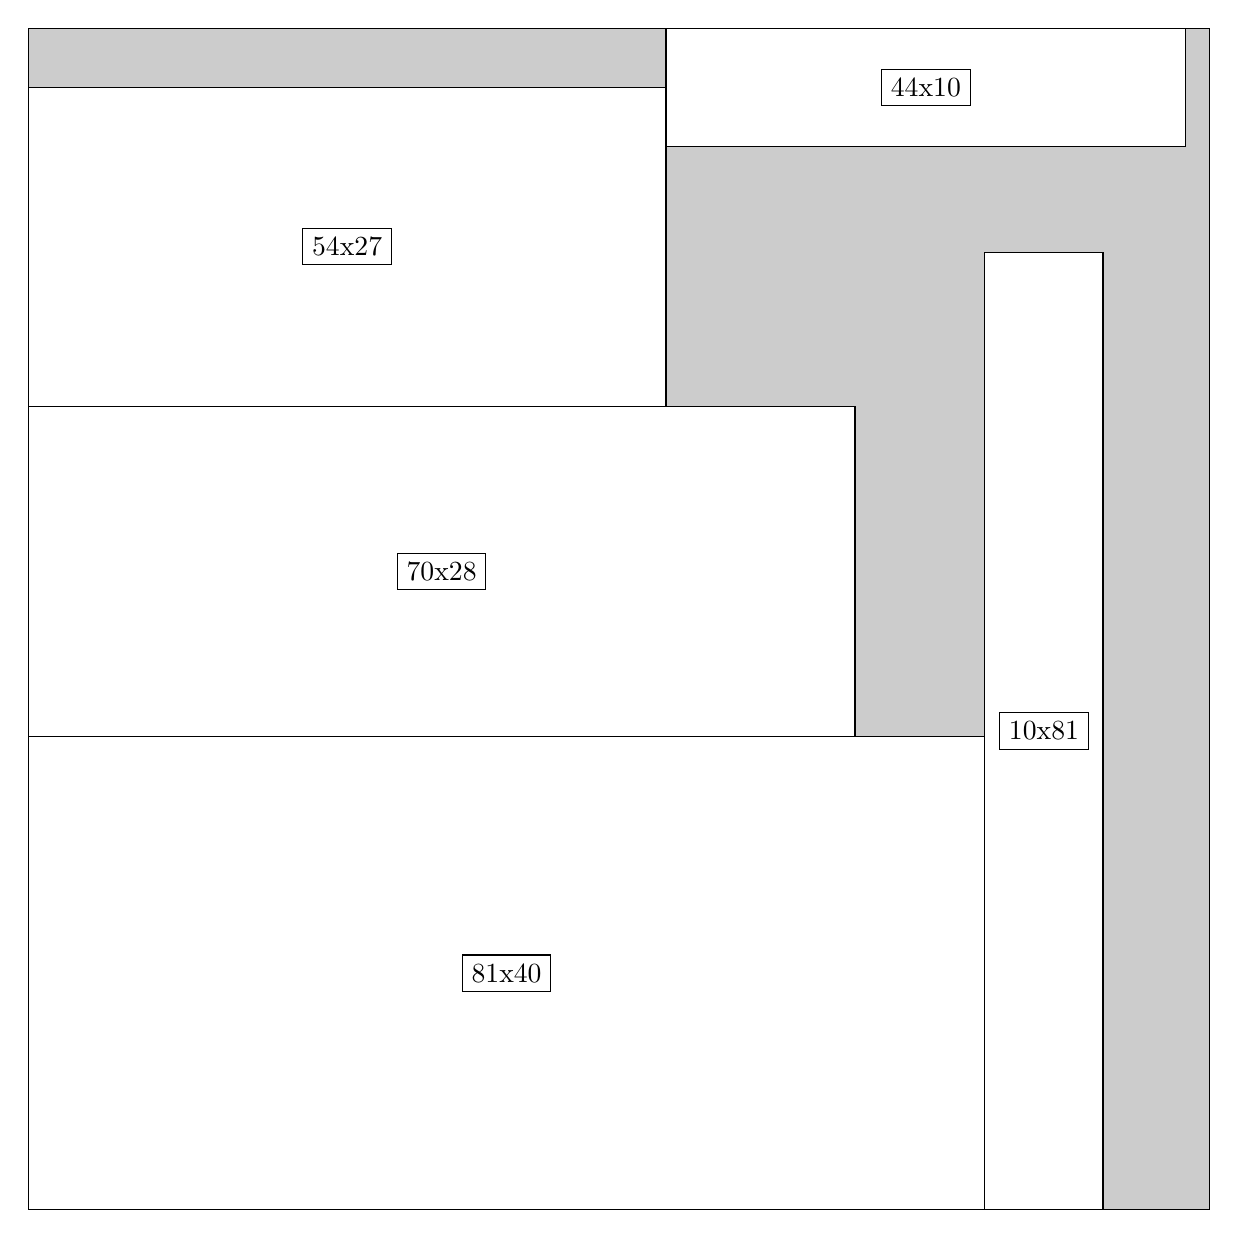
\begin{tikzpicture}[shorten >=1pt,scale=1.0,every node/.style={scale=1.0},->]
\tikzstyle{vertex}=[circle,fill=black!25,minimum size=14pt,inner sep=0pt]
\filldraw[fill=gray!40!white, draw=black] (0,0) rectangle (15.0,15.0);
\foreach \name/\x/\y/\w/\h in {81x40/0.0/0.0/12.15/6.0,70x28/0.0/6.0/10.5/4.2,54x27/0.0/10.2/8.1/4.05,10x81/12.15/0.0/1.5/12.15,44x10/8.1/13.5/6.6/1.5}
\filldraw[fill=white!40!white, draw=black] (\x,\y) rectangle node[draw] (\name) {\name} ++(\w,\h);
\end{tikzpicture}


w =81 , h =40 , x =0 , y =0 , v =3240
\par
w =70 , h =28 , x =0 , y =40 , v =1960
\par
w =54 , h =27 , x =0 , y =68 , v =1458
\par
w =10 , h =81 , x =81 , y =0 , v =810
\par
w =44 , h =10 , x =54 , y =90 , v =440
\par
\newpage


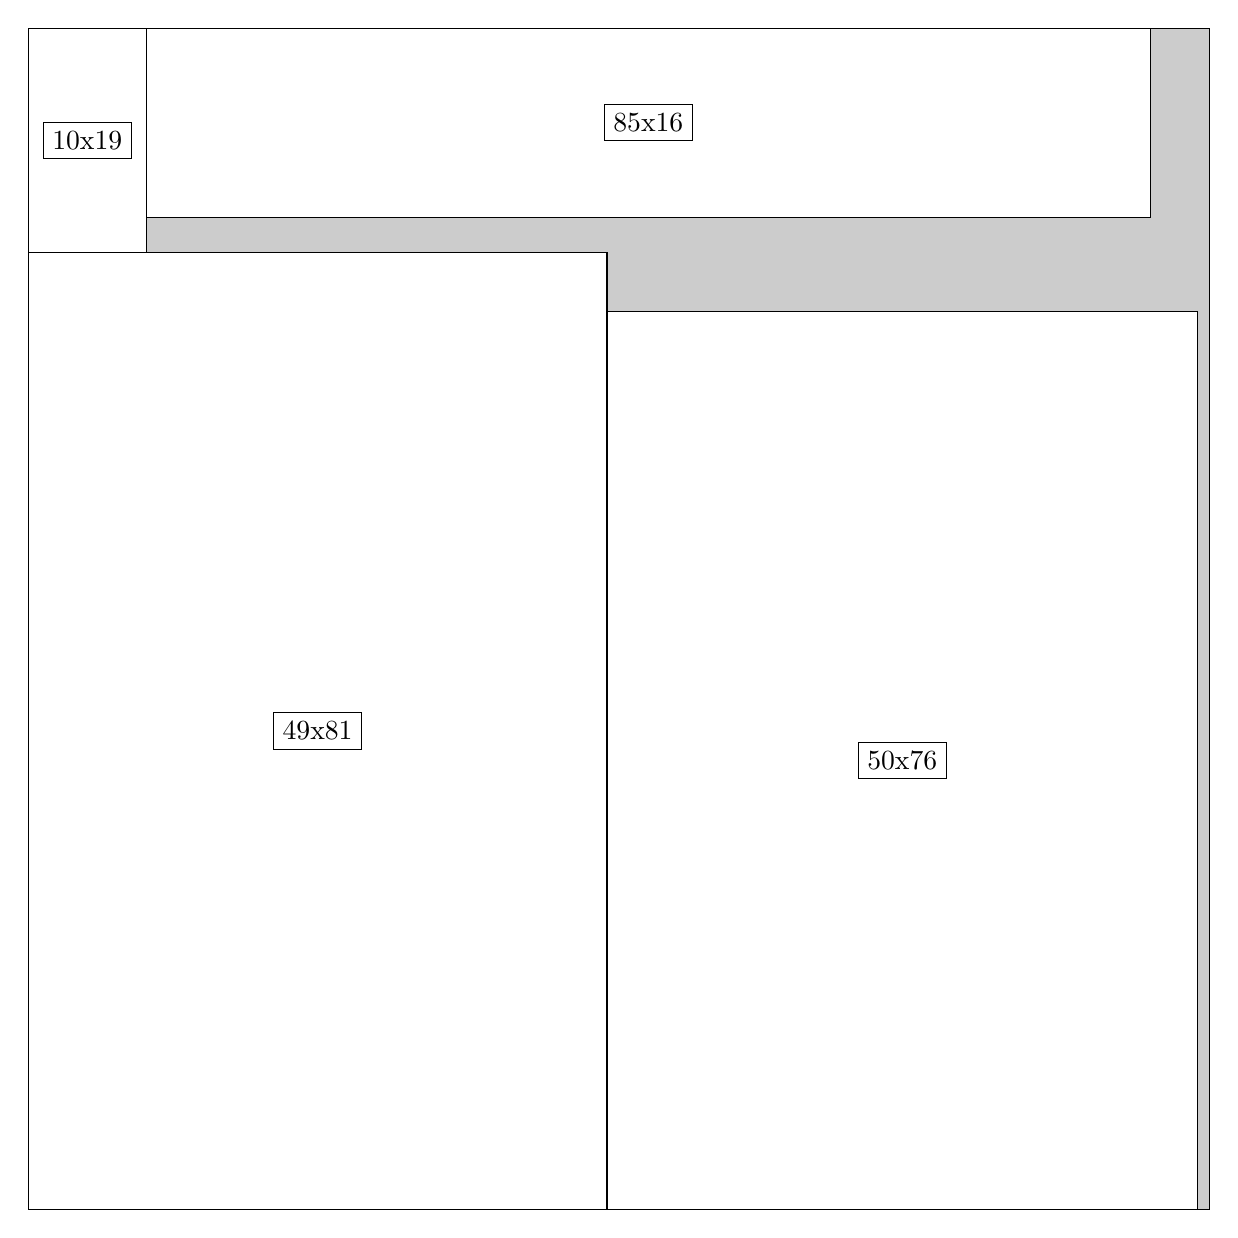
\begin{tikzpicture}[shorten >=1pt,scale=1.0,every node/.style={scale=1.0},->]
\tikzstyle{vertex}=[circle,fill=black!25,minimum size=14pt,inner sep=0pt]
\filldraw[fill=gray!40!white, draw=black] (0,0) rectangle (15.0,15.0);
\foreach \name/\x/\y/\w/\h in {49x81/0.0/0.0/7.35/12.15,50x76/7.35/0.0/7.5/11.4,85x16/1.5/12.6/12.75/2.4,10x19/0.0/12.15/1.5/2.85}
\filldraw[fill=white!40!white, draw=black] (\x,\y) rectangle node[draw] (\name) {\name} ++(\w,\h);
\end{tikzpicture}


w =49 , h =81 , x =0 , y =0 , v =3969
\par
w =50 , h =76 , x =49 , y =0 , v =3800
\par
w =85 , h =16 , x =10 , y =84 , v =1360
\par
w =10 , h =19 , x =0 , y =81 , v =190
\par
\newpage


\end{document}